

\chapter{Aproximação por mínimos quadrados}\label{cap_ajuste}
\thispagestyle{fancy}

\section{Problemas lineares}\label{cap_ajuste_sec_prob_lin}

Dado um conjunto de $n$ pontos $\{(x_i,y_i)\}_{i=1}^n$, $x_i\neq x_j$ para $i\neq j$, e uma família de $m \leq n$ funções $\{f_i(x)\}_{i=1}^m$, o problema linear de aproximação por mínimos quadrados consiste em determinar os $m$ coeficientes $\{c_i\}_{i=1}^m$ tal que a função
\begin{align}    
  f(x;c) &= \sum_{j=1}^m c_jf_j(x) \\
         &= c_1f_1(x) + c_2f_2(x) + c_3f_3(x) + \cdots + c_mf_m(x)
\end{align}
aproxime o conjunto de pontos dados no sentido de mínimos quadrados, i.e. o vetor dos coeficientes $c = (c_1, c_2, \dotsc, c_m)$ é solução do seguinte problema linear de minimização
\begin{equation}
  \min_{c} \left\{E:= \sum_{i=1}^n (y_i - f(x_i;c))^2\right\}.
\end{equation}

A fim de trabalharmos com uma notação mais compacta, definimos o resíduo $r(c) = (r_1(c), r_2(c), \dotsc, r_n(c))$, onde $r_i(c) := y_i - f(x_i)$ e $c = (c_1, c_2, \dotsc, c_m)$. Com esta notação, o problema de mínimos quadrados se resume a resolver
\begin{equation}\label{eq:pmq}
  \min_{c} \{E := \|r(c)\|_2^2\}.
\end{equation}

\subsection{Método das equações normais}

A fim de resolver o problema de mínimos quadrados~\eqref{eq:pmq}, observamos que o erro quadrático
\begin{align}
  E &= \|r(c)\|_2^2 \\
    &= \sum_{i=1}^n r_i(c)^2 \\
    &= \sum_{i=1}^n \left(y_i - f(x_i;c)\right)^2 \\
    &= \sum_{i=1}^n \left(y_i - \sum_{j=1}^m c_jf_j(x_i)\right)^2 \\
    &= \|y - Ac\|_2^2,
\end{align}
onde $y = (y_1, y_2, \dotsc, y_n)$ e
\begin{equation}
  A :=
  \begin{bmatrix}
    f_1(x_1) & f_2(x_1) & \cdots & f_m(x_1) \\
    f_1(x_2) & f_2(x_2) & \cdots & f_m(x_2) \\
    \vdots & \vdots & \vdots & \vdots \\
    f_1(x_n) & f_2(x_n) & \cdots & f_m(x_n)
  \end{bmatrix}.
\end{equation}

Os parâmetros $c_j$ que minimizam o erro $E$ são solução do seguinte sistema de equações
\begin{equation}
  \frac{\p E}{\p c_j} = 2\sum_{i=0}^n r_i(c)\frac{\p}{\p c_j}r_i(c) = 0,
\end{equation}
onde $j=1, 2, \dotsc, m$. Ou, em uma notação mais apropriada,
\begin{align}
  \nabla_c E = 0 &\Leftrightarrow A^Tr(c) = 0\\
  &\Leftrightarrow A^T(y - Ac) = 0\\
  &\Leftrightarrow A^TAc = A^Ty.
\end{align}

Portanto, o problema linear de mínimos quadrados se resume em resolver as chamadas \emph{equações normais}\index{equações normais}
\begin{equation}\label{eq:equacoes_normais}
  A^TAc= A^Ty.
\end{equation}

Logo, o problema linear de mínimos quadrados~\eqref{eq:pmq} reduz-se a resolver o sistema linear \eqref{eq:equacoes_normais} para $c$. Isto nos leva a questão de verificar se $A^TA$ é invertível. De sorte, da disciplina de álgebra linear temos o seguinte teorema.

\begin{teo}
  A matriz $A^TA$ é positiva definida se, e somente se, as colunas de $A$ são linearmente independentes (i.e. $\text{posto}(A)=n$).
\end{teo}
\begin{dem}
  Se as colunas de $A$ são linearmente independentes, então $x\neq 0$ implica $Ax\neq 0$ e, equivalentemente, $x^TA^T\neq 0$. Portanto, $x\neq 0$ implica $x^TA^TAx = \|Ax\|_2^2 > 0$, o que mostra que $A^TA$ é positiva definida.

  Suponhamos, agora, que as colunas de $A$ não são linearmente independentes. Então, existe $x_0\neq 0$ tal que $Ax_0 = 0$. Mas, então, $x_0^TA^TAx_0=0$, o que mostra que $A^TA$ não é positiva definida. 
\end{dem}

Este teorema nos fornece uma condição suficiente para a existência (e unicidade) de solução do problema linear de mínimos quadrados. Mais especificamente, se as colunas da matriz $A$ são linearmente independentes, então os coeficientes da função $f(x)$ que melhor ajustam os pontos dados são
\begin{equation}
  c = (A^TA)^{-1}A^Ty.
\end{equation}

\begin{ex}\normalfont{(Ajuste de polinômios)}\label{ex:ajuste_de_polinomios}
  Considere o problema de ajustar o conjunto de pontos
  \begin{center}
    \begin{tabular}{l|rrrr}
      $i$ & $1$ & $2$ & $3$ & $4$ \\\hline
      $x_i$ & $-1$ & $0$ & $1$ & $1,5$\\
      $y_i$ & $1,2$ & $-0,1$ & $0,7$ & $2,4$\\\hline
    \end{tabular}
  \end{center}
  por um polinômio quadrático da forma
  \begin{equation}
    p(x) = p_1x^2 + p_2x + p_3
  \end{equation}
  no sentido de mínimos quadrados.  

  \begin{figure}[h]
    \centering
    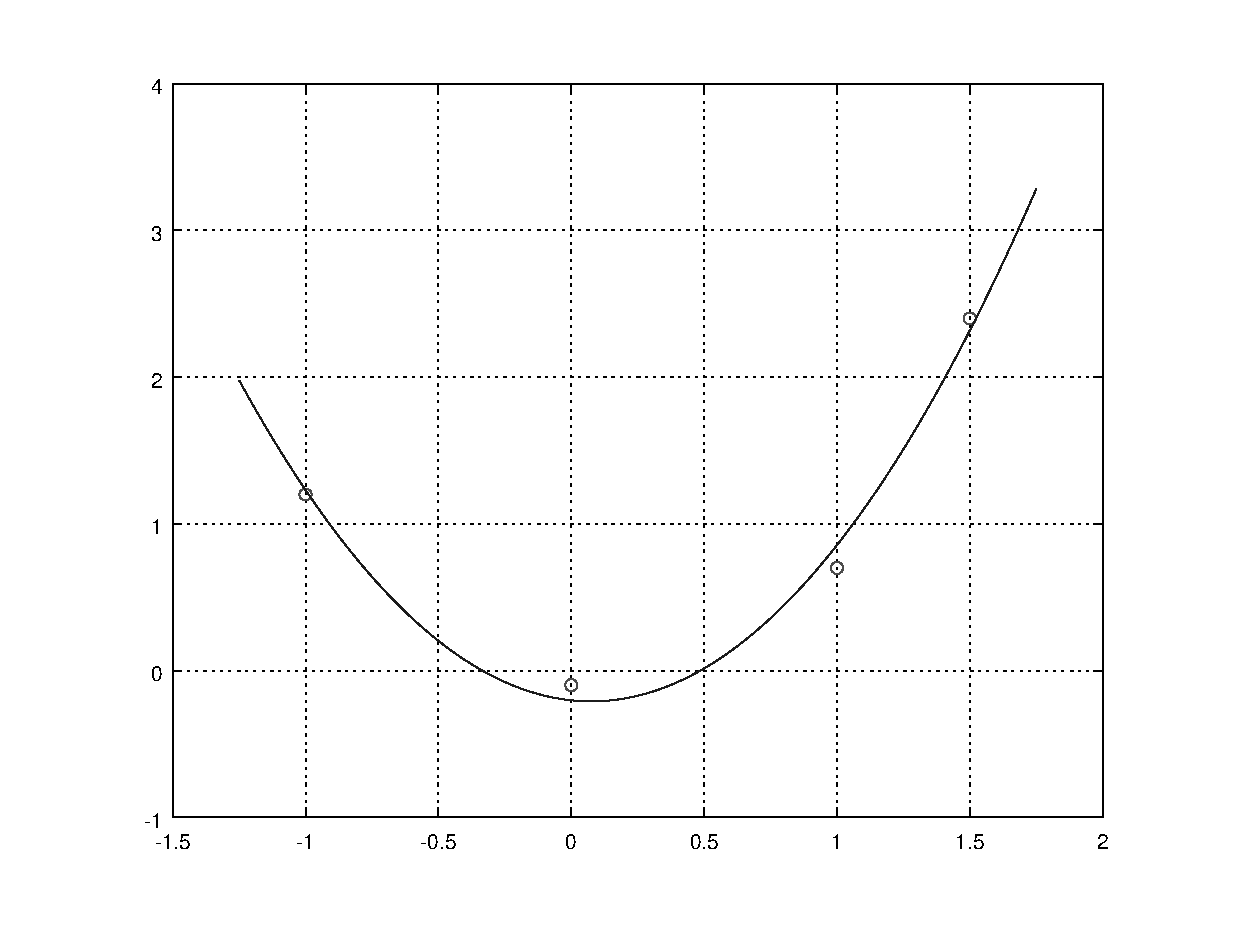
\includegraphics[width=\textwidth]{cap_ajuste/dados/ex_mq_poli/ex_mq_poli}
    \caption{Esboço do polinômio ajustado no Exemplo~\ref{ex:ajuste_de_polinomios}.}
    \label{fig:ex_mq_poli}
  \end{figure}
  
  
  Neste caso, a família de funções do problema de mínimos quadrados é $f_1(x) = x^2$, $f_2(x) = x$ e $f_3(x) = 1$. Assim sendo, os coeficientes $p = (p_1, p_2, p_3)$ são solução do seguinte sistema linear
  \begin{equation}\label{eq:aux3_md}
    A^TAp = A^Ty,
  \end{equation}
  onde $y = (y_1, y_2, y_3)$ e
  \begin{equation}
    A :=
    \begin{bmatrix}
      x_1^2 & x_1 & 1 \\
      x_2^2 & x_2 & 1 \\
      x_3^2 & x_3 & 1 \\
      x_4^2 & x_4 & 1
    \end{bmatrix}.
  \end{equation}
  Emfim, resolvendo as equações normais~\eqref{eq:aux3_md}, obtemos
  \begin{equation}
    p(x) = 1,25x^2 -0,188x - 0,203.
  \end{equation}
  A Figura~\ref{fig:ex_mq_poli} mostra um esboço dos pontos (em vermelho) e do polinômio ajustado (em azul).
  
  \ifisoctave
  Os coeficientes e um esboço do polinômio ajustado podem ser obtidos no \verb+GNU Octave+ com o seguinte código:
\begin{verbatim}
#pontos
x = [-1 0 1 1.5]';
y = [1.2, -0.1, 0.7, 2.4]';

#resol. as eqs. normais
A = [x.^2 x.^1 x.^0];
p = inv(A'*A)*A'*y

#esboco do pol. ajustado
xx = linspace(-1.25,1.75);
plot(x,y,'ro',...
     xx,polyval(p,xx));grid
\end{verbatim}
  \fi
  
\end{ex}


\begin{ex}\normalfont{(Ajuste de curvas)}\label{ex:ajuste_de_curvas}
  Consideremos o mesmo conjunto de pontos do exemplo anterior (Exemplo~\ref{ex:ajuste_de_polinomios}). Aqui, vamos ajustar uma curva da forma
  \begin{equation}
    f(x) = c_1\sen(x) + c_2\cos(x) + c_3
  \end{equation}
no sentido de mínimos quadrados. Para tanto, formamos a matriz
\begin{equation}
  A :=
  \begin{bmatrix}
    \sen(x_1) & \cos(x_1) & 1 \\
    \sen(x_2) & \cos(x_2) & 1 \\
    \sen(x_3) & \cos(x_3) & 1 \\
    \sen(x_4) & \cos(x_4) & 1
  \end{bmatrix}
\end{equation}
  e, então, resolvemos as equações normais $A^TAc = A^Ty$ para o vetor de coeficientes $c=(c_1, c_2)$. Fazendo isso, obtemos $c_1=-0,198$, $c_2=-2,906$ e $c_3=2,662$. A Figura~\ref{fig:ex_ajuste_de_curvas} mostra um esboço da curva ajustada (linha azul) aos pontos dados (círculos vermelhos).

  \begin{figure}[h]
    \centering
    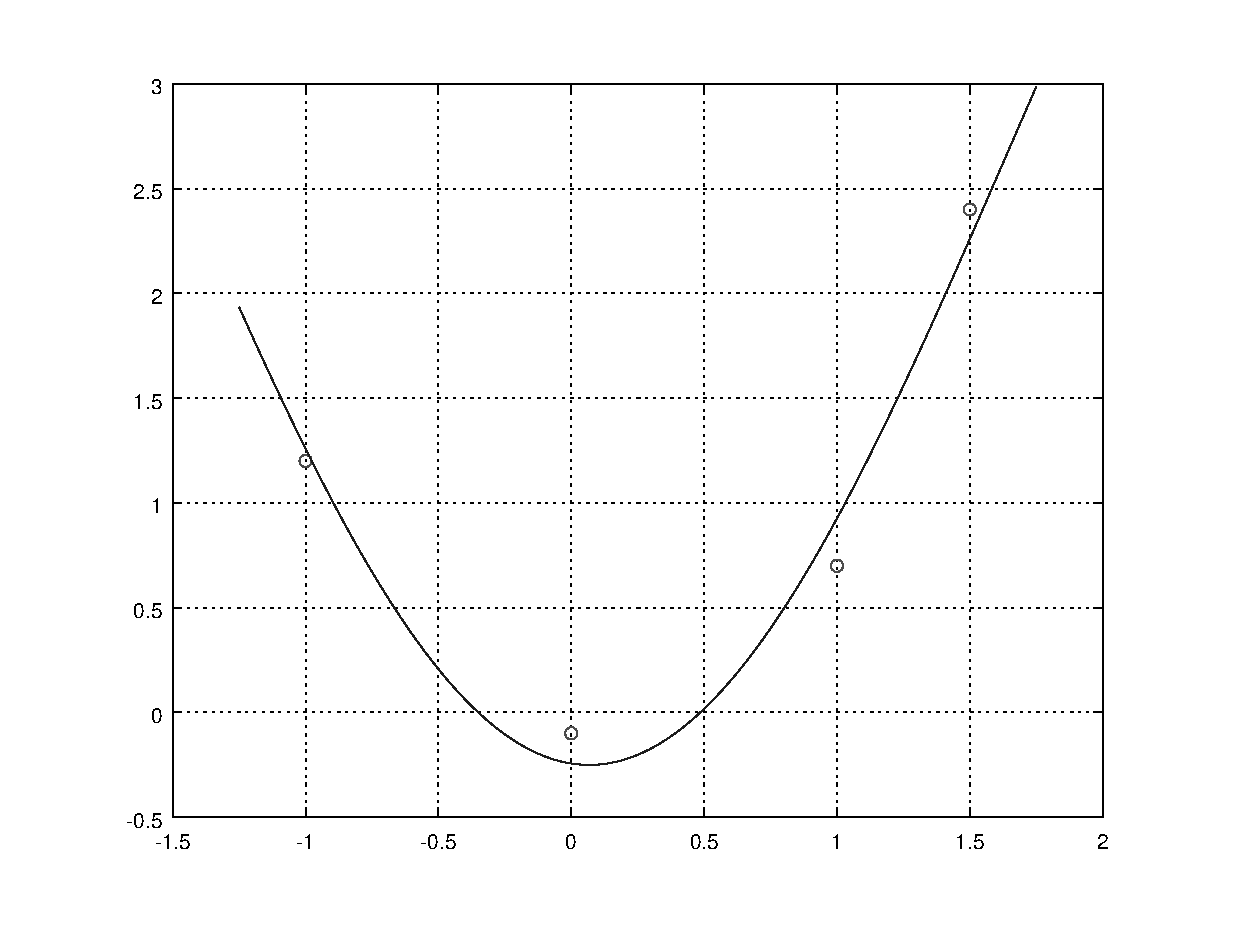
\includegraphics[width=\textwidth]{cap_ajuste/dados/ex_mq_curvas/ex_mq_curvas}
    \caption{Esboço da curva ajustada no Exemplo~\ref{ex:ajuste_de_curvas}.}
    \label{fig:ex_ajuste_de_curvas}
  \end{figure}

\ifisoctave
Os coeficientes e um esboço do polinômio ajustado podem ser obtidos no \verb+GNU Octave+ com o seguinte código:
\begin{verbatim}
#pontos
x = [-1 0 1 1.5]';
y = [1.2, -0.1, 0.7, 2.4]';

#resol. as eqs. normais
A = [sin(x) cos(x) ones(4,1)];
c = inv(A'*A)*A'*y

#curva ajustada
f = @(x) c(1)*sin(x) + c(2)*cos(x) + c(3)

#esboco da fun. ajustada
xx = linspace(-1.25,1.75);
plot(x,y,'ro',...
     xx,f(xx));grid
\end{verbatim}
\fi

\end{ex}

\begin{ex}\normalfont{(Um problema não linear)}\label{ex:mq_nlin0}
  Consideremos o problema de ajustar, no sentido de mínimos quadrados, à função
  \begin{equation}
    f(x) = c_1e^{c_2x}
  \end{equation}
ao seguinte conjunto de pontos
\begin{center}
  \begin{tabular}{l|rrrr}
    $i$ & $1$ & $2$ & $3$ & $4$ \\\hline
    $x_i$ & $-1$ & $0$ & $1$ & $1,5$\\
    $y_i$ & $8,0$ & $1,5$ & $0,2$ & $0,1$\\\hline
  \end{tabular}
\end{center}

Aqui, temos um problema não linear de mínimos quadrados que pode ser transformado em um problema linear fazendo-se
\begin{align}
  y = c_1e^{c_2x} &\Rightarrow \ln y = \ln c_1e^{c_2x}\\
                  &\Rightarrow \ln y = \ln c_1 + c_2x.
\end{align}
Isto é, denotando $d_1 := \ln c_1$ e $d_2 := c_2$, o problema se resume a ajustar uma reta $r(x) = d_1 + d_2x$ ao conjunto de pontos $\{(x_i, \ln y_i)\}_{i=1}^4$. 

Para resolver o problema transformado, formamos a matriz
\begin{equation}
  A :=
  \begin{bmatrix}
    1 & x_1 \\
    1 & x_2 \\
    1 & x_3 \\
    1 & x_4
  \end{bmatrix}
\end{equation}
e, então, resolvemos as equações normais $A^TAd = A^T\ln y$, com $\ln y = (\ln y_1, \ln y_2, \ln y_3, \ln y_4)$, donde obtemos $d_1=0,315$ e $d_2=-1,792$. Das definições de $d_1$ e $d_2$, temos $c_2 = d_2 = -1,792$ e $c_1 = e^{d_1} = 1,371$. A Figura~\ref{fig:ex_mq_nlin0} mostra um esboço da curva $f(x) = c_1e^{c_2x}$ ajustada (linha azul) aos pontos dados (círculos vermelhos).

\begin{figure}[h]
  \centering
  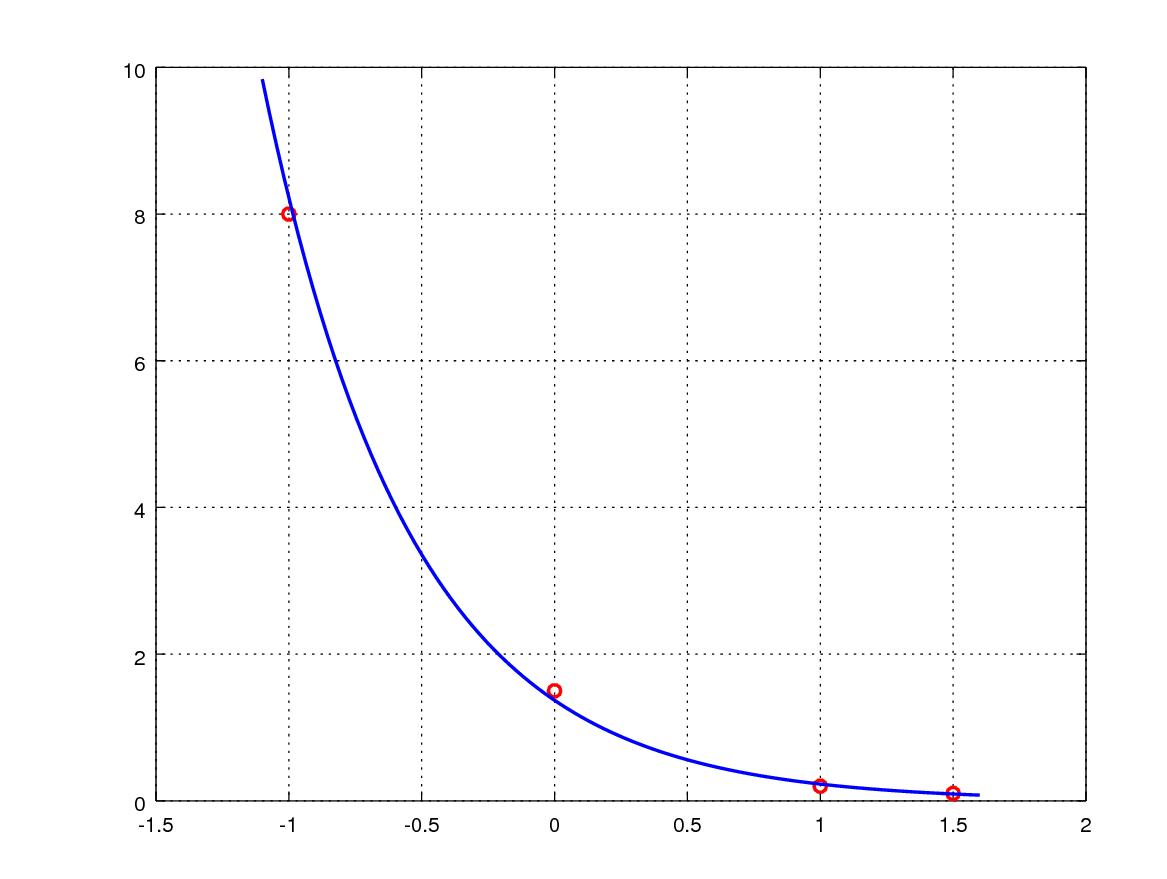
\includegraphics[width=\textwidth]{cap_ajuste/dados/ex_mq_nlin0/ex_mq_nlin0}
  \caption{Esboço da curva ajustada no Exemplo~\ref{ex:mq_nlin0}.}
  \label{fig:ex_mq_nlin0}
\end{figure}

\ifisoctave
O ajuste e um esboço da função ajustada podem ser feitos no \verb+GNU Octave+ com o seguinte código:
\begin{verbatim}
#pontos
x = [-1 0 1 1.5]';
y = [8.0 1.5 0.2 0.1]';

#resol. as eqs. normais
A = [ones(4,1) x];
d = inv(A'*A)*A'*log(y)

#fun. ajustada
c = [exp(d(1)); d(2)]
f = @(x) c(1)*exp(c(2)*x);

#esboco da fun. ajustada
xx = linspace(-1.1,1.6);
plot(x,y,'ro','linewidth',1.5,...
     xx,f(xx),'b-','linewidth',1.5);grid
\end{verbatim}
\fi

\end{ex}

\subsection*{Exercícios}

\begin{exer}\label{exer:mq_reta}
  Determine a reta $y = c_1x + c_2$ que melhor se ajusta, no sentido de mínimos quadrados, aos pontos
  \begin{center}
    \begin{tabular}{l|ccccc}
      $i$ & $1$ & $2$ & $3$ & $4$ & $5$ \\\hline
      $x_i$ & $-2,5$ & $-1,3$ & $0,2$ & $1,7$ & $2,3$\\
      $y_i$ & $3,8$ & $1,5$ & $-0,7$ & $-1,5$ & $-3,2$\\\hline
    \end{tabular}
  \end{center}
Por fim, compute a norma $L^2$ do resíduo, i.e. $\|r(c)\|_2 = \|y - (c_1x - c_2)\|_2$ para os pontos dados.
\end{exer}
\begin{resp}
  \ifisoctave 
  \href{https://github.com/phkonzen/notas/blob/master/src/MatematicaNumerica/cap_ajuste/dados/exer_mq_reta/exer_mq_reta.m}{Código.} 
  \fi
  $c_1 = -1,3259$, $c_2 = 8,66071\E-2$, $\|r(c)\|_2 = 1,01390$.
\end{resp}

\begin{exer}\label{exer:mq_poli}
  Determine o polinômio $y = c_1x^3 + c_2x^2 + c_3x + c_4$ que melhor se ajusta, no sentido de mínimos quadrados, aos pontos
  \begin{center}
    \begin{tabular}{l|ccccc}
      $i$ & $1$ & $2$ & $3$ & $4$ & $5$ \\\hline
      $x_i$ & $-2,5$ & $-1,3$ & $0,2$ & $1,7$ & $2,3$\\
      $y_i$ & $3,8$ & $0,5$ & $2,7$ & $1,2$ & $-1,3$\\\hline
    \end{tabular}
  \end{center}
Por fim, compute a norma $L^2$ do resíduo, i.e. $\|r(c)\|_2$.
\end{exer}
\begin{resp}
  \ifisoctave 
  \href{https://github.com/phkonzen/notas/blob/master/src/MatematicaNumerica/cap_ajuste/dados/exer_mq_poli/exer_mq_poli.m}{Código.} 
  \fi
  $c_1 = -4,50361\E-1$, $c_2 = -2,78350\E-1$, $c_3 = 1,46291$, $c_4 = 2,09648$, $\|r(c)\|_2 = 5,71346$
\end{resp}

\begin{exer}\label{exer:mq_curva}
  Determine a curva $y = c_1\sen x + c_2\cos x + c_3$ que melhor se ajusta, no sentido de mínimos quadrados, aos pontos
  \begin{center}
    \begin{tabular}{l|ccccc}
      $i$ & $1$ & $2$ & $3$ & $4$ & $5$ \\\hline
      $x_i$ & $-2,5$ & $-1,3$ & $0,2$ & $1,7$ & $2,3$\\
      $y_i$ & $3,8$ & $0,5$ & $2,7$ & $1,2$ & $-1,3$\\\hline
    \end{tabular}
  \end{center}
Por fim, compute a norma $L^2$ do resíduo, i.e. $\|r(c)\|_2$.
\end{exer}
\begin{resp}
  \ifisoctave 
  \href{https://github.com/phkonzen/notas/blob/master/src/MatematicaNumerica/cap_ajuste/dados/exer_mq_curva/exer_mq_curva.m}{Código.} 
  \fi
  $c_1 = -2,76842$, $c_2 = -7,17935\E-1$, $c_3 = 1,37014\E-1$, $\|r(c)\|_2 = 2,48880\E+1$
\end{resp}

\begin{exer}\label{exer:mq_nlin0}
  Use a transformação $z = \ln y$ para ajustar, no sentido de mínimos quadrados, a curva $y = c_1e^{c_2(x-c_3)^2}$ aos pontos
  \begin{center}
    \begin{tabular}{l|cccccc}
      $i$ & $1$ & $2$ & $3$ & $4$ & $5$ & $6$ \\\hline
      $x_i$ & $-0,5$ & $0,5$ & $1,3$ & $2,1$ & $2,7$ & $3,1$ \\
      $y_i$ & $0,1$ & $1,2$ & $2,7$ & $0,9$ & $0,2$ & $0,1$ \\\hline
    \end{tabular}
  \end{center}
\end{exer}
\begin{resp}
  \ifisoctave 
  \href{https://github.com/phkonzen/notas/blob/master/src/MatematicaNumerica/cap_ajuste/dados/exer_mq_nlin0/exer_mq_nlin0.m}{Código.} 
  \fi
  $c_1 = 2,10131\E+0$, $c_2 = -9,73859\E-1$, $c_3 = 1.25521\E+0$
\end{resp}
   
\section{Problemas não lineares}\label{cap_ajuste_sec_prob_nlin}

Um problema não linear de mínimos quadrados consiste em ajustar uma dada função $f(x;c)$ que dependa não linearmente dos parâmetros $c = (c_1, c_2, \dotsc, c_m)$, $m\geq 1$, a um dado conjunto de $n\geq m$ pontos $\{(x_i, y_i)\}_{i=1}^n$. Mais especificamente, buscamos resolver o seguinte problema de minimização
\begin{equation}\label{eq:prob_nlin_mq}
  \min_{\{c_1, c_2, \dotsc, c_m\}} \left[E := \sum_{i=1}^n \left(y_i - f(x_i;c)\right)^2\right].
\end{equation}
Aqui, denotaremos por $r(c) := (r_1(c), r_2(c), \dotsc, r_n(c))$ o vetor dos resíduos $r_i(c) := y_i - f(x_i,c)$. Com isso, o problema se resume a encontrar o vetor de parâmetros $c$ que minimiza
\begin{equation}
  E = \|r(c)\|_2^2.
\end{equation}
Tais parâmetros são solução do seguinte sistema de equações
\begin{equation}
  \frac{\p E}{\p c_j} = 2\sum_{i=1}^n r_i(c)\frac{\p}{\p c_j}r_i(c) = 0
\end{equation}
ou, equivalentemente, da equação
\begin{equation}\label{eq:grad_E}
  \nabla E = 0 \Leftrightarrow J_R^T(c)r(c) = 0,
\end{equation}
onde
\begin{equation}
  J_R(c) :=
  \begin{bmatrix}
    \frac{\p r_1}{\p c_1} & \frac{\p r_1}{\p c_2} & \cdots & \frac{\p r_1}{\p c_m}\\
    \frac{\p r_2}{\p c_1} & \frac{\p r_2}{\p c_2} & \cdots & \frac{\p r_2}{\p c_m}\\
    \vdots  & \vdots & \vdots & \vdots \\
    \frac{\p r_n}{\p c_1} & \frac{\p r_n}{\p c_2} & \cdots & \frac{\p r_n}{\p c_m}
  \end{bmatrix}
\end{equation}
é a jacobiana do resíduo $r$ em relação aos parâmetros $c$.

Podemos usar o método de Newton para resolver~\eqref{eq:grad_E}. Para tanto, escolhemos uma aproximação inicial para $c^{(1)} = (c_1^{(1)}, c_2^{(1)}, \dotsc, c_m^{(1)})$ e iteramos
\begin{align}
  H_R(c^{(k)})\delta^{(k)} &= -J_R^T(c)r(c) \label{eq:mqnl_newton1}\\
  c^{(k+1)} &= c^{(k)} + \delta^{(k)} \label{eq:mqnl_newton2},
\end{align}
onde $\delta^{(k)} = (\delta_1^{(k)}, \delta_2^{(k)}, \delta_m^{(k)})$ é a atualização de Newton (ou direção de busca) e $H_R(c) := [h_{p,q}(c)]_{p,q=1}^{m,m}$ é a matriz hessiana, cujos elementos são
\begin{equation}
  h_{p,q} := \sum_{i=1}^n\left\{\frac{\p r_i}{\p c_q}\frac{\p r_i}{\p c_p} + r_i\frac{\p^2 r_i}{\p c_q\p c_p}\right\}.
\end{equation}

\begin{ex}\label{ex:mqnl_newton}
  Consideremos o problema de ajustar, no sentido de mínimos quadrados, a função
  \begin{equation}
    f(x;c) = c_1e^{c_2x}
  \end{equation}
ao seguinte conjunto de pontos
\begin{center}
  \begin{tabular}{l|rrrr}
    $i$ & $1$ & $2$ & $3$ & $4$ \\\hline
    $x_i$ & $-1$ & $0$ & $1$ & $1,5$\\
    $y_i$ & $8,0$ & $1,5$ & $0,2$ & $0,1$\\\hline
  \end{tabular}
\end{center}

Aqui, vamos utilizar a iteração de Newton para o problema de mínimos quadrados, i.e. a iteração dada em \eqref{eq:mqnl_newton1}-\eqref{eq:mqnl_newton2}. Para tanto, para cada $i=1, 2, 3, 4$, precisamos das seguintes derivadas parciais do resíduo $r_i(c) := y_i - c_1e^{c_2x_i}$:
\begin{align}
  &\frac{\p}{\p c_1}r_i(c) = - e^{c_2x_i},\\
  &\frac{\p}{\p c_2}r_i(c) = - c_1x_ie^{c_2x_i},\\
  &\frac{\p^2}{\p c_1^2}r_i(c) = 0,\\
  &\frac{\p^2}{\p c_1\p c_2}r_i(c) = \frac{\p^2}{\p c_2\p c_1}r_i(c) = - x_ie^{c_2x_i},\\
  &\frac{\p^2}{\p c_2^2}r_i(c) = - c_1x_i^2e^{c_2x_i}.
\end{align}

\begin{figure}[h]
  \centering
  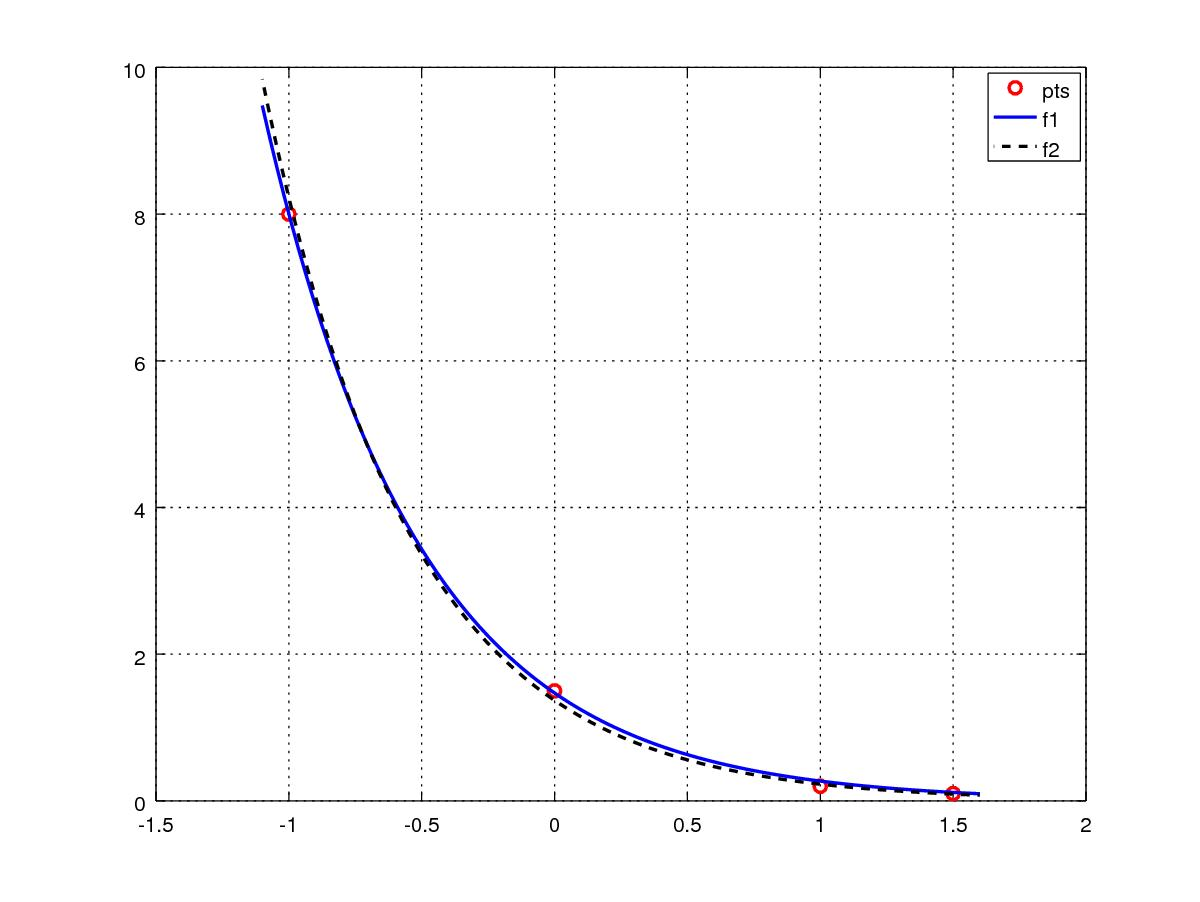
\includegraphics[width=\textwidth]{cap_ajuste/dados/ex_mqnl_N/ex_mqnl_N}
  \caption{Esboço da curva ajustada no Exemplo~\ref{ex:mqnl_newton}.}
  \label{fig:ex_mqnl_newton}
\end{figure}

Com isso e tomando $c^{(1)} = (1,4, ~-1,8)$ (motivado do Exemplo~\ref{ex:mq_nlin0}), computamos as iterações de Newton~\eqref{eq:mqnl_newton1}-\eqref{eq:mqnl_newton2}. Iterando até a precisão de $TOL = 10^{-4}$, obtemos a solução $c_1 = 1,471$ e $c_2 = -1,6938$. Na Figura~\ref{fig:ex_mqnl_newton} vemos uma comparação entre a curva aqui ajustada ($-$) e aquela obtida no Exemplo~\ref{ex:mq_nlin0} ($--$).

\ifisoctave
O ajuste discutido neste exemplo pode ser computado no \verb+GNU Octave+ com o seguinte código:
\begin{verbatim}
#pontos
global x = [-1 0 1 1.5]';
global y = [8.0 1.5 0.2 0.1]';

#fun. objetivo
f = @(x,c) c(1)*exp(c(2)*x);

#residuo
r = @(c) y - f(x,c);

#jacobiana
function A = J(c)
  global x
  A = zeros(4,2);
  A(:,1) = - exp(c(2)*x);
  A(:,2) = - c(1)*x.*exp(c(2)*x);
endfunction

#hessiana
function A = H(c)
  global x
  global y
  A = zeros(2,2);
  A = J(c)'*J(c);
  for i=1:4
    A(1,1) += 0;
    A(1,2) += (y(i) - c(1)*exp(c(2)*x(i))) * ...
              (- x(i)*exp(c(2)*x(i)));
    A(2,1) += (y(i) - c(1)*exp(c(2)*x(i))) * ...
              (- x(i)*exp(c(2)*x(i)));
    A(2,2) += (y(i) - c(1)*exp(c(2)*x(i))) * ...
              (- c(1)*x(i)^2*exp(c(2)*x(i)));
  endfor
endfunction

#aprox. inicial
c = [1.4 -1.8]';

#iteracoes de Newton
k=0;
do
  k+=1;
  delta = - inv(H(c))*J(c)'*r(c);
  c = c + delta;
  [k,c',norm(delta)]
until ((k>10) | (norm(delta)<1e-4))
\end{verbatim}
\fi
\end{ex}

Observamos que a solução obtida no exemplo anterior (Exemplo~\ref{ex:mqnl_newton}) difere da previamente encontrada no Exemplo~\ref{ex:mq_nlin0}. Naquele exemplo, os parâmetros obtidos nos fornecem $E = 6,8\E-2$, enquanto que a solução do exemplo anterior fornece $E = 6,1\E-3$. Isto é esperado, pois naquele exemplo resolvemos um problema aproximado, enquanto no exemplo anterior resolvemos o problema por si.

O emprego do método de Newton para o problema de mínimos quadrados tem a vantagem da taxa de convergência quadrática, entretanto requer a computação das derivadas parciais de segunda ordem do resíduo. Na sequência discutimos alternativas comumente empregadas.

\subsection{Método de Gauss-Newton}

O método de Gauss-Newton é uma técnica iterativa que aproxima o problema não linear de mínimos quadrados \eqref{eq:prob_nlin_mq} por uma sequência de problemas lineares. Para seu desenvolvimento, começamos de uma aproximação inicial $c^{(1)} = (c_1^{(1)}, c_2^{(1)}, \dotsc, c_m^{(1)})$ dos parâmetros que queremos ajustar. Também, assumindo que a $n$-ésima iterada $c^{(k)}$ é conhecida, faremos uso da aproximação de primeira ordem de $f(x,c)$ por polinômio de Taylor, i.e.
\begin{equation}
  f(x;c^{(k+1)}) \approx f(x;c^{(k)}) + \nabla_c f(x;c^{(k)})(c^{(k+1)}-c^{(k)}),
\end{equation}
onde
\begin{equation}
  \nabla_c f(x;c) = \left[\frac{\p}{\p c_1}f(x;c) ~\frac{\p}{\p c_2}f(x;c) ~\cdots ~\frac{\p}{\p c_m}f(x;c)\right].
\end{equation}

O método consiste em obter a solução do problema não linear \eqref{eq:prob_nlin_mq} pelo limite dos seguintes problemas lineares de mínimos quadrados
\begin{align}
  \min_{\delta^{(k)}} &\left[\tilde{E} := \sum_{i=1}^n (y_i - f(x_i,c^{(k)}) - \nabla_c f(x_i;c^{(k)})\delta^{(k)})^2\right] \label{eq:mq_gn0}\\
  &c^{(k+1)} = c^{(k)} + \delta^{(k)}.
\end{align}

Agora, usando a notação de resíduo $r(c) = y - f(x;c)$, observamos que \eqref{eq:mq_gn0} consiste no problema linear de mínimos quadrados
\begin{equation}
  \min_{\delta^{(k)}} \|r(c^{(k)}) + J_R(c^{(k)})\delta^{(k)}\|_2^2,
\end{equation}
o qual é equivalente a resolver as equações normais
\begin{equation}
  J_R^T(c^{(n)})J_R(c^{(n)})\delta^{(n)} = -J_R^T(c)r(c).
\end{equation}

Com isso, dada uma aproximação inicial $c^{(1)}$, a \emph{iteração do método de Gauss-Newton} consiste em
\begin{align}
  &J_R^T(c^{(k)})J_R(c^{(k)})\delta^{(k)} = -J_R^T(c)r(c)\\
  &c^{(k+1)} = c^{(k)} + \delta^{(k)}.
\end{align}

\begin{ex}
  A aplicação da iteração de Gauss-Newton ao problema de mínimos quadrados discutido no Exemplo~\ref{ex:mqnl_newton} nos fornece a mesma solução obtida naquele exemplo (preservadas a aproximação inicial e a tolerância de precisão).

\ifisoctave
A implementação do método de Gauss-Newton para este problema no \verb+GNU Octave+ pode ser feita com o seguinte código:
\begin{verbatim}
#pontos
global x = [-1 0 1 1.5]';
y = [8.0 1.5 0.2 0.1]';

#fun. objetivo
f = @(x,c) c(1)*exp(c(2)*x);

#residuo
r = @(c) y - f(x,c);

#jacobiana
function A = J(c)
  global x
  A = zeros(4,2);
  A(:,1) = - exp(c(2)*x);
  A(:,2) = - c(1)*x.*exp(c(2)*x);
endfunction

#aprox. inicial
c = [1.4 -1.8]';

#iteracoes de Gauss-Newton
k=0;
do
  k+=1;
  delta = - inv(J(c)'*J(c))*J(c)'*r(c);
  c = c + delta;
  [k,c',norm(delta)]
until ((k>10) | (norm(delta)<1e-4))
\end{verbatim}
\fi
\end{ex}

O método de Gauss-Newton pode ser lentamente convergente para problemas muito não lineares ou com resíduos grandes. Nesse caso, métodos de Gauss-Newton com amortecimento são alternativas robustas~\cite{Bjorck1996a,Nocedal2006a}. Na sequência, introduziremos um destes métodos, conhecido como método de Levenberg-Marquardt.

\subsection{Método de Levenberg-Marquardt}

O método de Levenberg-Marquardt é uma variação do método de Gauss-Newton no qual a direção de busca $\delta^{(n)}$ é obtida da solução do seguinte problema regularizado
\begin{equation} \label{eq:mq_gn0}
  \min_{\delta^{(k)}} \{\|r(c^{(k)}) + J_R(c^{(k)})\delta^{(k)}\|_2^2 + \mu^{(k)}\|\delta^{(k)}\|_2^2\}
\end{equation}
ou, equivalentemente,
\begin{equation} \label{eq:mq_gn0}
  \min_{\delta^{(k)}} \left\|
    \begin{bmatrix}
      r(c^{(k)})\\
      0
    \end{bmatrix} +
    \begin{bmatrix}
      J_R(c^{(k)})\\
      \mu^{(k)}I
    \end{bmatrix}
    \delta^{(k)}\right\|_2^2
\end{equation}

A taxa de convergência das iterações de Levenberg-Marquardt é sensível a escolha do parâmetro $\mu^{(k)}\geq 0$. Aqui, faremos esta escolha por tentativa e erro. O leitor pode aprofundar-se mais sobre esta questão na literatura especializada (veja, por exemplo, \cite{Bjorck1996a,Nocedal2006a}).

\begin{obs}
  Quando $\mu^{(k)} \equiv 0$ para todo $n$, o método de Levenberg-Marquardt é equivalente ao método de Gauss-Newton.
\end{obs}

\begin{ex}\label{ex:mqnl_LM}
  Consideremos o problema de mínimos quadrados discutido no Exemplo~\ref{ex:mqnl_newton}. O método de Gauss-Newton falha para este problema se escolhermos, por exemplo, $c^{(1)} = (0, 0)$. Isto ocorre pois, para esta escolha de $c^{(1)}$, a jacobiana $J(c^{(1)})$ não tem posto completo. Entretanto, o método de Levenberg-Marquardt com $\mu^{(k)} = 0,1$ é convergente, mesmo para esta escolha de $c^{(1)}$.

\ifisoctave
A implementação no \verb+GNU Octave+ do método de Levenberg-Marquardt (com $\mu^{(k)}=0,1$ constante) para este problema pode ser feita com o seguinte código:
\begin{verbatim}
#pontos
global x = [-1 0 1 1.5]';
y = [8.0 1.5 0.2 0.1]';

#fun. objetivo
f = @(x,c) c(1)*exp(c(2)*x);

#residuo
r = @(c) y - f(x,c);

#jacobiana
function A = JR(c)
  global x;
  A = zeros(4,2);
  A(:,1) = - exp(c(2)*x);
  A(:,2) = - c(1)*x.*exp(c(2)*x);
endfunction

#aprox. inicial
c = [0 0]';

#param. de amortecimento
mu = 0.1;

#iteracoes de Gauss-Newton
k=0;
do
  k+=1;
  JJ = [JR(c);mu*eye(2,2)];
  delta = - inv(JJ'*JJ)*JJ'*[r(c);zeros(2,1)];
  c = c + delta;
  printf("%d %1.1e %1.3e %1.3e\n", k,norm(delta),c')
until ((k>10) | (norm(delta)<1e-4))
\end{verbatim}
\fi
\end{ex}

\subsection*{Exercícios}

\begin{exer}\label{exer:mqnl_GN}
  Use o método de Gauss-Newton para ajustar, no sentido de mínimos quadrados e com precisão de $10^{-4}$, a curva $y = c_1e^{c_2(x-c_3)^2}$ aos pontos
  \begin{center}
    \begin{tabular}{l|cccccc}
      $i$ & $1$ & $2$ & $3$ & $4$ & $5$ & $6$ \\\hline
      $x_i$ & $-0,5$ & $0,5$ & $1,3$ & $2,1$ & $2,7$ & $3,1$ \\
      $y_i$ & $0,1$ & $1,2$ & $2,7$ & $0,9$ & $0,2$ & $0,1$ \\\hline
    \end{tabular}
  \end{center}
Use as condições iniciais:
\begin{enumerate}[a)]
\item $c_1 = 2,1$, $c_2=-1$ e $c_3=1,3$.
\item $c_1=1$, $c_2=-1$ e $c_3=-1$.
\end{enumerate}
\end{exer}
\begin{resp}
  \ifisoctave 
  \href{https://github.com/phkonzen/notas/blob/master/src/MatematicaNumerica/cap_ajuste/dados/exer_mqnl_GN/exer_mqnl_GN.m}{Código.} 
  \fi
  a) $c_1 = 2,69971\E+0$, $c_2 = -1,44723\E+0$, $c_3 = 1.24333\E+0$; b) divergente.
\end{resp}

\begin{exer}
  Resolva o exercício anterior (Exercício~\ref{exer:mqnl_GN}) usando o método de Levenberg-Marquardt com amortecimento constante $\mu=0,2$.
\end{exer}
\begin{resp}
  \ifisoctave 
  \href{https://github.com/phkonzen/notas/blob/master/src/MatematicaNumerica/cap_ajuste/dados/exer_mqnl_LM/exer_mqnl_LM.m}{Código.} 
  \fi
  a)  $c_1 = 2,69971\E+0$, $c_2 = -1,44723\E+0$, $c_3 = 1.24333\E+0$; b) $c_1 = 2,69971\E+0$, $c_2 = -1,44723\E+0$, $c_3 = 1.24333\E+0$
\end{resp}
